\documentclass[10pt,a4paper,twoside]{article}
% The following LaTeX packages must be installed on your machine: amsmath, authblk, bm, booktabs, caption, dcolumn, fancyhdr, geometry, graphicx, hyperref, latexsym, natbib

% Please make sure that spp.dat (supplied with this template) is in your working directory or path
\input{spp.dat}

%  Editorial staff will uncomment the next line
% \providecommand{\artnum}[0]{XX-XX}
% \renewcommand{\articlenum}[0]{SPP-\the\year-\artnum-}

\usepackage{adjustbox}

\begin{document}

%--------------------------------------------------
%  Fill in the paper's title in Sentence case
%  Titles beginning with articles (A, An, The) are discouraged
%--------------------------------------------------
\title{\TitleFont Virtual Kulintang prototype using computer vision}


%--------------------------------------------------
% For TWO authors with the same affiliation please use this block
% Or Please use the other author block templates
%--------------------------------------------------
%\author[*\negthickspace]{Author M.~Surname}
%\author[ ]{Bauthor D.~Surname~III
%\lastauthorsep}
%\affil[ ]{Department of Science, XXX University, Country}
%\affil[*]{\corremail{amsurname@university.edu} }

%--------------------------------------------------
%  For three or more authors with the same affiliation please use this block
%--------------------------------------------------

% \author[*]{Author M.~Surname\authorsep}
% \author[ ]{Bauthor D.~Surname~Jr.\authorsep}
% \author[ ]{Cauthor D.~Surname~III\lastauthorsep}
% \affil[ ]{Department of Science, XXX University, Country}
% \affil[*]{\corremail{amsurname@university.edu} }

%--------------------------------------------------
%  For authors with different affiliations please use the following block
%--------------------------------------------------
 \author[1*]{Christian James E.~Barimbao~\authorsep}
 \author[1]{Martina Joanna A.~Manuel~\authorsep}
 \author[1]{Claire Joy H.~Ramos~\authorsep}
 \author[1]{Carl Timothy S. ~Tolentino~\authorsep}
% % !!! Please take note that the last author separation is \lastauthorsep instead of \authorsep
 \author[2]{Maricor N.~Soriano~\lastauthorsep}
 \affil[1]{Electrical and Electronics Engineering Institute, University of the Philippines Diliman, Philippines}
 \affil[2]{Natinal Institute of Physics, University of the Philippines Diliman, Philippines}
 \affil[*]{\corremail{christian.barimbao@eee.upd.edu.ph} }


\begin{abstract}
\noindent
%--------------------------------------------------
% Include abstract and keywords here
%--------------------------------------------------
Philippine indigenous instruments, especially the Kulintang, face challenges related to cost, availability, and transportation. We developed a virtual Kulintang that exploits image processing techniques in Python's OpenCV to simulate the playing mechanics of the instrument using colored markers.  Our goal is to introduce users to this instrument and further preserve its cultural significance. The system successfully detects and tracks the centroid of these markers, averaging 24 frames per second (FPS), while closely resembling the physical instrument's overall layout. 

\keywords{kulintang, digital musical instruments, computer vision, image processing}

\end{abstract}

\maketitle
\thispagestyle{titlestyle}


%--------------------------------------------------
% the main text of your paper begins here
%--------------------------------------------------
\section{Introduction}\label{sec:intro}
Philippine indigenous musical instruments and the manner of playing them are representative of the rich culture specific to certain tribes. The Kulintang is an indigenous instrument native to the Mindanao islands in the southern part of the country. It consists of a set of eight embossed gongs suspended horizontally on two parallel strings arranged from largest to smallest, left to right, as seen in Figure \ref{fig:Kulintangan}.

According to a personal interview with a Kulintang master at the University of the Philippines (UP) Center for Ethnomusicology, interest in Philippine indigenous musical instruments has been declining due to the high cost and limited availability of manufacturers, making procurement and learning difficult (A. Butocan, Professor, College of Music, UP Diliman, Dec. 6, 2022). This is especially true for the Kulintang, which is also challenging to transport. In this work, we aim to develop a prototype of a virtual Kulintang instrument using low-cost distinct-colored markers, a laptop webcam, and synthesized Kulintang sounds. While virtual instruments aim to bridge the inaccessibility of their physical counterparts, current applications mostly focus on western-based instruments like the drums \cite{tolentino_air_2019}, guitar \cite{karjalainen_virtual_2006, pakarinen_virtual_2008, tamani_building_2018}, and violin \cite{Fan2013}. Although some locally-inspired virtual instruments exist, most of them rely on touch-based feedback, which bears little resemblance to the actual playing mechanics of the instrument \cite{tanfelix_virtual_2020, baltazar_digital_2020, lucas_digital_2013}.

Our algorithm employs standard image processing techniques, including histogram backprojection, dilation, and thresholding -- implemented using the Python OpenCV library. We aim to develop a prototype that generates sound output upon the markers' tracked position hitting the bounding boxes, simulating the play of a Kulintang. This work attempts to contribute to the appreciation and preservation of Philippine indigenous music by making a virtual prototype of Kulintang that will be easily accessible to the end users.

\begin{figure}[h!]
\centering
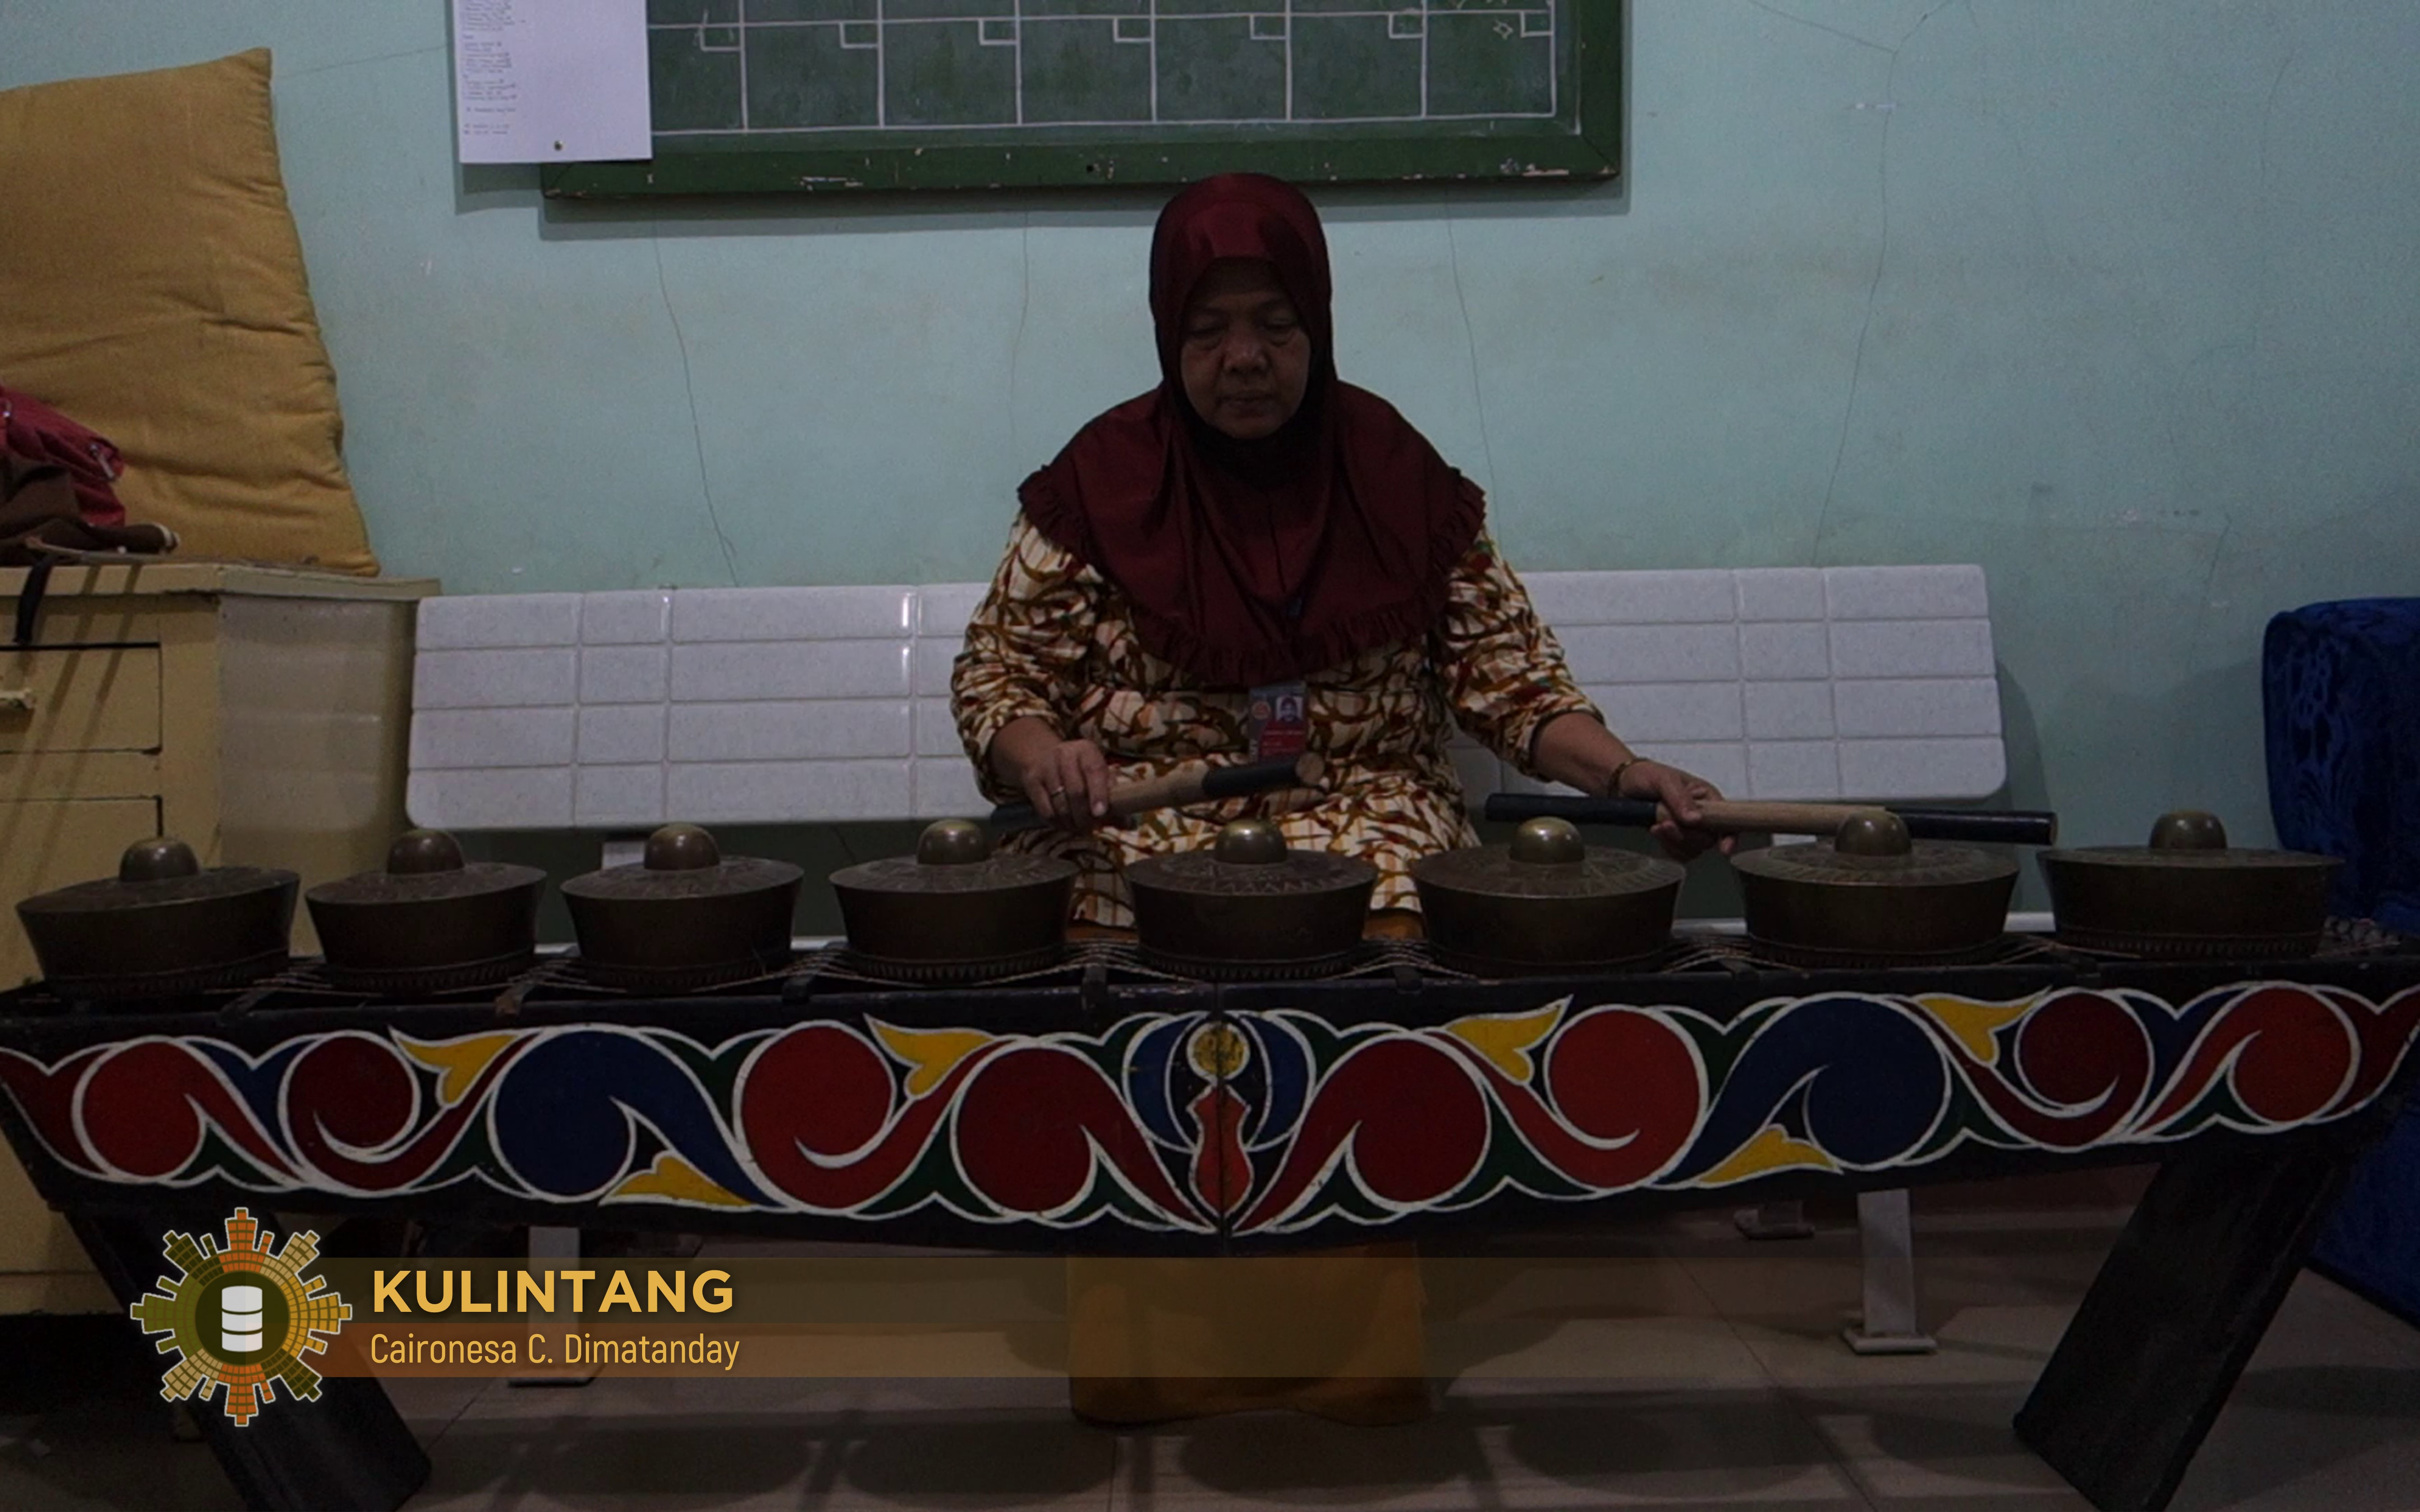
\includegraphics[width=0.34\textwidth]{MR_KULINTANG.jpeg}\label{fig:kulintang}
\quad % or other spacing between figures
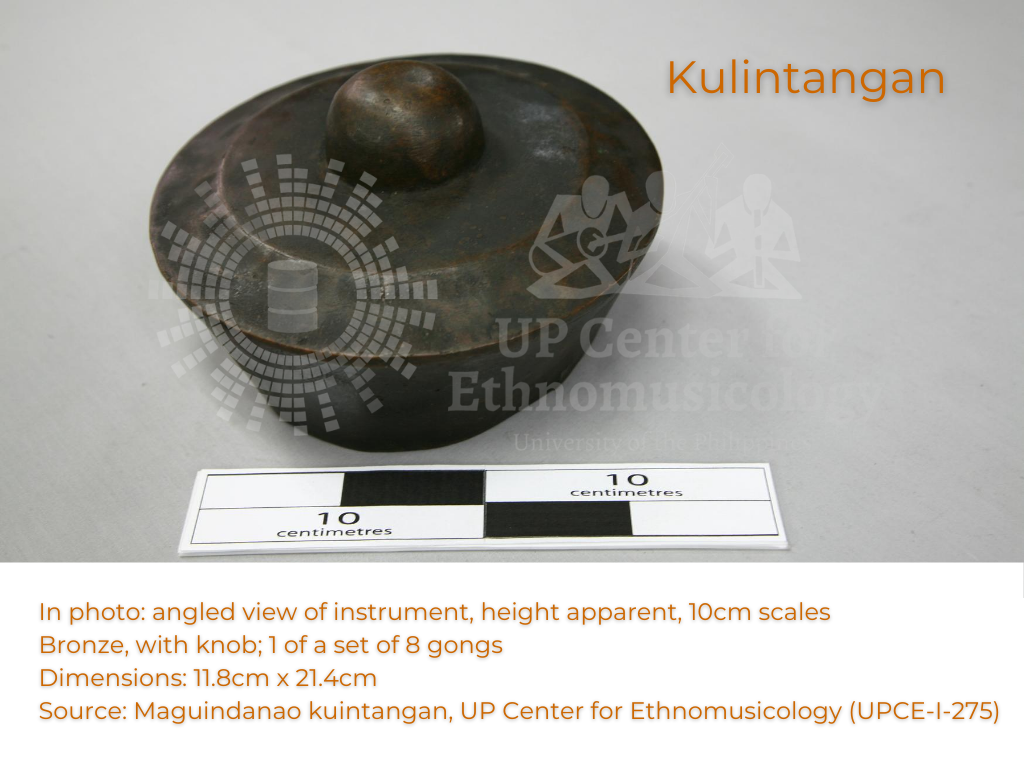
\includegraphics[width=0.28\textwidth]{Kulintangan (275b).png}\label{fig:gong}
\caption{The Kulintang gongs are knobbed at the center and played using a pair of soft wooden sticks called the \emph{basal}. Source of images: Department of Science and Technology-Advanced Science and Technology Institute (DOST-ASTI) Project Katunog \cite{philippine_copyright_2023_by_dost-asti_and_up_kulintang_2019, philippine_copyright_2023_by_dost-asti_and_up_kulintangan_2019}.}
\label{fig:Kulintangan}
\end{figure}



\section{Methodology}\label{sec:methodology}

\subsection{Calibration}\label{sec:calibration} 
At the beginning of the program, the user is prompted to calibrate the system for initial use as shown in Figure \ref{fig:calibration}. The calibration involves positioning each colored marker within the bounding circle, which serves as the region of interest (ROI), and clicking the mouse to cue the program to crop the ROI and obtain the Red, Green, and Blue (RGB) values per pixel of the markers. The maximum and minimum RGB values are also stored for thresholding later (\ref{sec:blob_detection}). Subsequently, the RGB values are converted to the Normalized Chromaticity Coordinates (NCC) using the following equations:

\begin{equation}
    \centering
    I = R + G + B, \quad
    r = R/I, \quad
    g = G/I
\end{equation}{}

where $I$ represents the pixel intensity, and  $(r,g)$ are the NCC coordinate values. Normalizing with intensity reduces the effect of brightness on the chromaticity values $r$ and $g$. Finally, the 2D-histogram of the ROI with the NCC is computed and normalized to one. Histogram values lesser than 0.5 will be rounded to zero.


\begin{figure}[t!]
    \centering
    \begin{tabular}{cc} 
    \adjustbox{valign=b}{\begin{tabular}{@{}c@{}}
    \subfloat[Red marker calibration\label{subfig-2:TaclobanNorth}]{%
          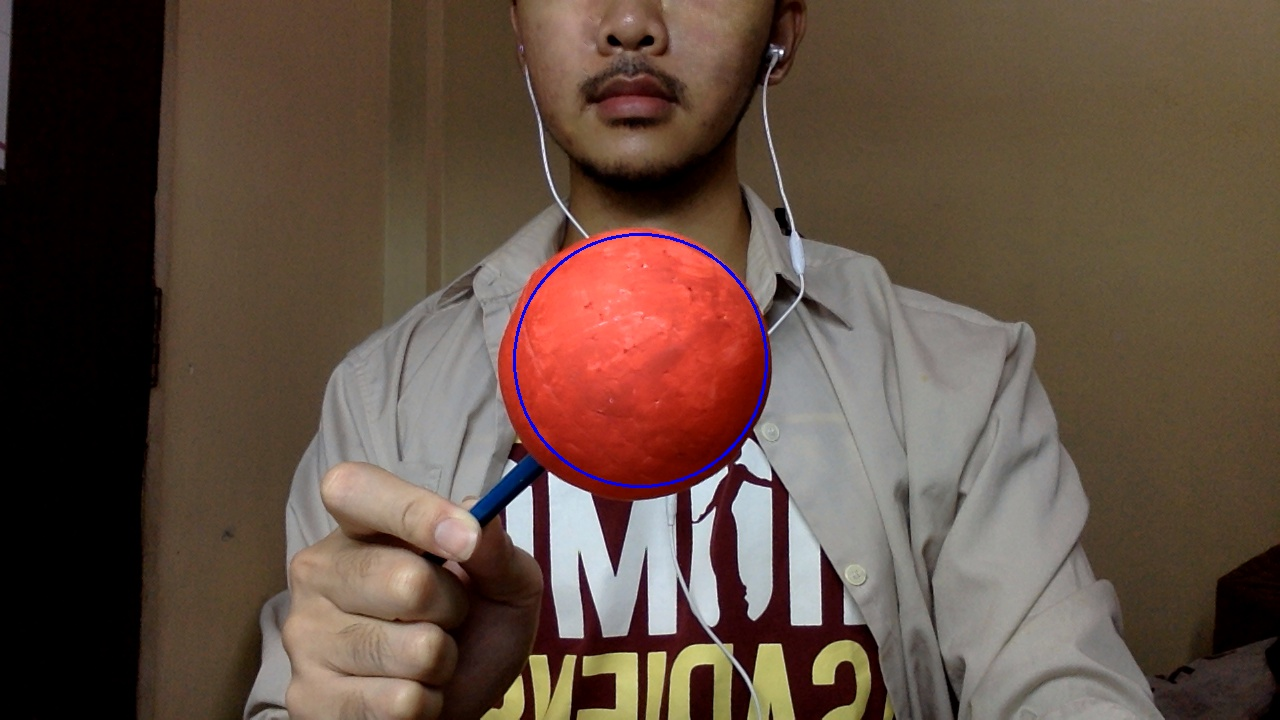
\includegraphics[width=.25\linewidth]{calibration_red.jpeg}} \\
    \subfloat[Green marker calibration\label{subfig-3:LeyteResettlement}]{%
          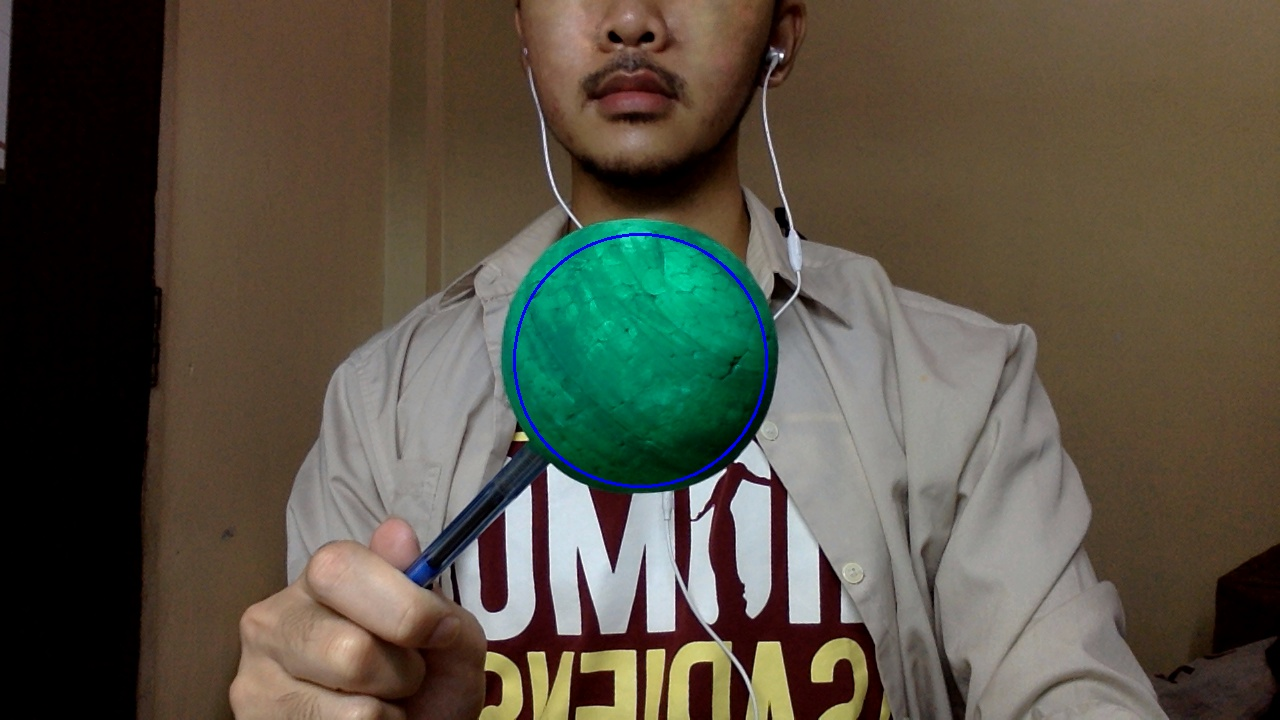
\includegraphics[width=.25\linewidth]{calibration_green.jpeg}}
    \end{tabular}}
    &
    \adjustbox{valign=b}{\subfloat[2D-histogram of the ROI\label{subfig-1:2d-hist}]{
\includegraphics[width=.38\linewidth]{histogram.png}}}
    \end{tabular}
    \caption{The 2D-histogram of the colored markers is obtained from the cut-out regions during calibration.}\label{fig:calibration}
\end{figure}

\subsection{Blob Detection}\label{sec:blob_detection}



\begin{figure}[b!]
    \centering
    \subfloat[Red ROI]{
\includegraphics[width=0.18\textwidth]{segmented_r.png}\label{fig:segment_r}}
    \quad % or other spacing between figures
    \subfloat[Green ROI]{
\includegraphics[width=0.18\textwidth]{segmented_g.png}\label{fig:segment_g}}
    \quad % or other spacing between figures
    \subfloat[Dilated red ROI]{
\includegraphics[width=0.18\textwidth]{blob_r.png}\label{fig:blob_r}}
    \quad % or other spacing between figures
    \subfloat[Dilated green ROI]{
\includegraphics[width=0.18\textwidth]{blob_g.png}\label{fig:blob_g}}
    \quad % or other spacing between figures
    \subfloat[Centroid Estimation]{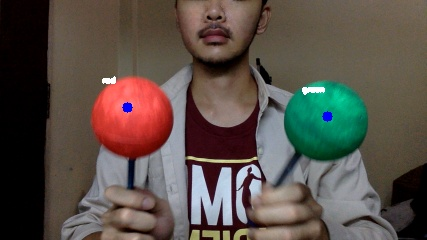
\includegraphics[width=0.4\textwidth]{centroid.jpeg}\label{fig:centroid}}

  \caption{Blob detection algrotihm. The input frame is segmented using histogram backprojection then dilated to fill pixel gaps in the blob before calculating for the centroid.}\label{fig:blob-detection}
\end{figure}


In order to segment the images, histogram backprojection is employed, since a simple table lookup algorithm is proven advantageous in real-time applications \cite{soriano_adaptive_2003}. For each pixel $p_{i}$ of the subsequent input images, a value $S_{i}(r_{i}, g_{i})$  will be assigned, where  $S(r,g)$ corresponds to the histogram values calculated in \ref{sec:calibration}. Histogram backprojection is appropriate to use for real-time robust color detection since it is fast enough while being insensitive to shading and lighting variations. In this work, we used a bin size of $32$ but different bin size resolutions can be set to cater different applications. Higher bin size usually means more fine-grained color segmentation while lower bin size allows more color variations.

Then, the backprojected image will be thresholded using the stored maximum and minimum $RGB$ values in calibration to further remove background artifacts.  This results to a segmented image, as demonstrated in Figures \ref{fig:segment_r} and 
\ref{fig:segment_g}. 

The segmented image is then dilated to increase the blob size and improve centroid estimation, as observed in Figures \ref{fig:blob_r} and \ref{fig:blob_g}. The centroid is computed using the center of mass formula with $m_i = 1$:
\begin{equation}
    \centering
    \bar{x} = \dfrac{\sum\limits_{i=1}^n x_i m_i}{\sum\limits_{i=1}^n m_i},
    \quad
    \bar{y} = \dfrac{\sum\limits_{i=1}^n y_i m_i}{\sum\limits_{i=1}^n m_i}
\end{equation}{}

where $n$ is the total number of white pixels, $x_i$ and $y_i$ are the indices of the $i$-th pixel, and $\bar{x}$ and $\bar{y}$ are the coordinates of the centroid.

\subsection{Hit Detection and Gong Playback}
The event of a gong being hit is determined by the comparison of each marker's current position to its position in the previous frame, and a corresponding boolean variable called \emph{hit-state}. The \emph{hit-state} is initialized to \emph{False} for both markers during startup, and will assert to \emph{True} when the centroid goes inside a bounding box. The \emph{hit-state} will then become \emph{False} for the succeeding frames that the centroid remains inside the bounding box to prevent infinite triggers. The $x$ value of the centroid during a \emph{hit-state = True} will determine which gong sound will play. A strike of a gong for each marker is displayed in Figure \ref{fig:hit-detect} 

\begin{figure}[tbp]
    \centering
    \subfloat[Strike: Green Marker]{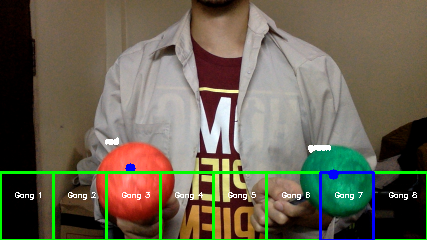
\includegraphics[width=0.33\textwidth]{strike_g.png}}\label{fig:hit_green}
    \quad 
    % or other spacing between figures
    \subfloat[Strike: Red Marker]{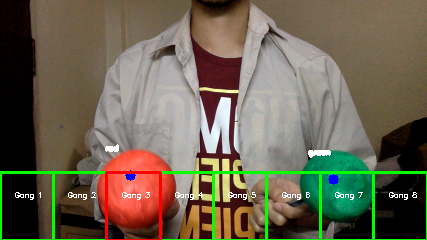
\includegraphics[width=0.33\textwidth]{strike_r.png}}\label{fig:hit_red}
    \caption{Hit Detection.}\label{fig:hit-detect}
\end{figure}



\section{Results and Discussion}
The system was tested using colored Styro balls as markers attached to the ends of a pen. It can be noted that the algorithm was still able to detect and track the centroid of irregularly shaped objects like rectangular plastic containers, handheld fans, and  bottles. However, a spherical object is preferred for simplicity and to ensure invariance to the camera viewing angle. Red and green colors were used as they were readily available, but it can be safely assumed that any contrasting colors will work. 

During initial tests, it was observed that the system achieved an average execution time between frames of 43 milliseconds or approximately 24 FPS, which is the standard for real-time video applications. The performance can be further improved in the future through additional code optimizations (e.g. multi-threading, employing graphical processing unit (GPU) methods, etc.). The lighting conditions also seem to affect the processing speed, with images captured in darker environments exhibiting slower processing times. This can be attributed to the increased noise and lower contrast in low-light images resulting in a greater number of digital artifacts. 

The overall sample layout is presented in Figure \ref{fig:system}. A video demonstration of the system can also be viewed from this link (\href{https://youtu.be/pTm6Q4q3aAE}{youtu.be/pTm6Q4q3aAE}). The software decision of the layout of the gongs is intentional to resemble the actual physical instrument. Because of this, there are constraints on the user's mobility while playing the virtual instrument. With the achievement of real-time motion tracking, we can now calculate kinematical quantities such as the velocity and acceleration of the basal. This shall be integrated on the sound synthesis to generate more realistic sounds. It must be reiterated  however, that the ultimate goal of our work is simply to open new avenues for appreciating the Kulintang, or as a tool to introduce it to beginners, and not as a means to replace the actual instrument.

\begin{figure}[h!]
  \centering
  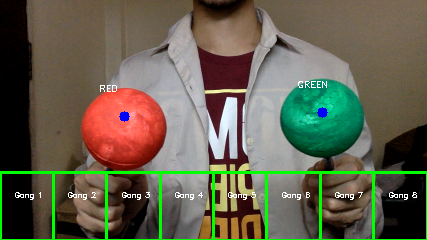
\includegraphics[width=0.40\textwidth]{system.png}
  \caption{System Overview. Each box is arranged in increasing pitch, analogous to the actual gongs.}
  \label{fig:system}
\end{figure}

\section{Conclusions}
We have successfully developed a virtual Kulintang prototype that utilizes computer vision techniques for synthesizing gong sounds. Future work includes enhancing sound synthesis with marker acceleration tracking and improving the application's graphical interface. These advancements aim to provide a more immersive and user-friendly experience for musicians and enthusiasts, paving the way for further advancements in virtual instruments and the preservation of traditional music.

\section*{Acknowledgments}
All gong sounds and images used in this work are a property of the DOST \emph{Katunog} project. Philippine Copyright 2023 by DOST-ASTI and UP \cite{philippine_copyright_2023_by_dost-asti_and_up_katunog_2019}.

% Please use the style file spp-bst.bst. If you wish to use BibTeX, kindly use us the filename bibfile.bib for your bib file.
\bibliographystyle{spp-bst}
\bibliography{bibfile}

\end{document}